\section{Rircerca dell'involucro
convesso}\label{rircerca-dellinvolucro-convesso}

Si ha un insieme di punti e si vuole trovare il più piccolo involucro
convesso che li contiene tutti.

\subsection{Algortimo di Graham}\label{algortimo-di-graham}

Se l'insieme \emph{Q} contiene \emph{n} punti riesce a risolvere il
problema in \emph{O(n log n)}.

L'algoritmo inizia cercando il punto \emph{p0} più in basso. Se ci sono
più punti con la stessa \emph{y} minima, effettua il tie-breaking
prendendo quello più a sinistra.

Dopodiché ordina i restanti \emph{n-1} punti per angolo polare rispetto
a \emph{p0} e se due punti hanno lo stesso ancorlo polare li ordina per
distanza crescente da \emph{p0}

Una volta stabilito l'ordinamento dei punti \emph{p0 p1 \ldots{} pn-1},
l'algoritmo inizia a costruire incrementalmente l'involucro convesso
utilizzando una struttura dati \emph{S} che si comporta come una pila.

Su \emph{S} è possibile eseguri:

\begin{itemize}
\tightlist
\item
  \texttt{Push(S,p)}: aggiunge il punto \emph{p} in cima alla pila
\item
  \texttt{Pop(S)}: elimina il primo elemento della pila
\item
  \texttt{Top(S)}: restituisce, senza eliminarlo, il valore del primo
  elemento della pila
\item
  \texttt{Next-To-Top(S)}: restituisce il valore del penultimo elemento
  della pila.
\end{itemize}

L'algoritmo inizia inserendo \emph{p0} nella pila, \emph{p0} è
sicuramente un punto dell'involucro convesso perché è quello più a in
basso a sinistra. Quindi quando c'è solo \emph{p0} in \emph{S} si ha
l'involucro convesso degenere.

Dopodiché per ogni punto restante l'algoritmo prova ad aggiungerlo nel
poligono convesso. Quando viene aggiunto un nuovo punto viene fatto un
controllo per rimuovere da \emph{S} i punti che sono interni.

Questo viene fatto considerando i primi due punti della pila, \emph{p} e
\emph{q}, e il punto corrente \emph{p\_i}.

Da notare che se nella pila c'è un solo elemento, il punto \emph{pi}
viene aggiunto senza problemi, perché in quel momento non può essere
interno.

Se nel passare dal segmento \emph{qp} al segmento \emph{ppi} c'è una
svolta a destra, vuol dire che aggiungendo il punto \emph{pi} al
poligono, il punto \emph{p} diventa interno e quindi deve essere tolto.

Una volta tolto \emph{p} è necessario rieffettuare lo stesso controllo,
perché può essere che anche \emph{q} diventi un punto interno del
poligono.

\begin{verbatim}
Graham-Scan(Q)
    cerca p0
    ordina p1, ... pn-1 per angolo polare rispetto a p0
    \State \textsc{Push}$(S,p_0)$
    \For{$i = 1 \textbf{ to } n-1$}
        \State $p \gets \textsc{Top}(S)$
        \State $q \gets \textsc{Next-To-Top}(S)$
         \While{$q \neq \textsc{Nil} \textbf{ and } \textsc{Turn-left}(q,p,p_i)$}
            \State \textsc{Pop}$(S)$
            \State $p \gets q$
            \State $q \gets \textsc{Next-To-Top}(S)$
         \EndWhile
         \State Push(S,p_i)
    \EndFor
    \State \Return $S$
\end{verbatim}

Per dimostrare la \textbf{correttezza} dell'algoritmo è necessario
dimostrare che un punto viene tolto dal poligono solo quando non
appartiene\ldots{}.

Discorso dell'angolo polare\ldots{}

\begin{figure}[htbp]
\centering
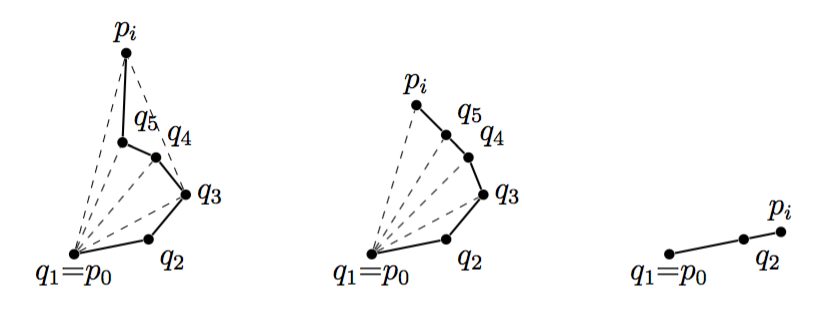
\includegraphics{./immagini/l32-fig1.png}
\caption{}
\end{figure}

La \textbf{complessità} dell'algortimo ha un \emph{O(n)} per la ricerca
di \emph{p\_0}, \emph{O(n log n)} per l'ordinamento dei punti e un
restante \emph{O(n)} per l'esecuzione del for. La complessità totale è
quindi dominata da quella della ricerca.

\subsection{Algoritmo di Jarvis}\label{algoritmo-di-jarvis}

L'algoritmo di Jarvis calcola l'involucro convesso in tempo \emph{O(nh)}
dove \emph{h} è il numero di vertici.

L'idea alla base dell'algorimto è quella di andare a \emph{recitare dei
chiodi piantati su un pezzo di legno con uno spago legato ad un punto
del poligono convesso}.

L'algoritmo cerca quindi il punto \emph{p0} in modo analogo
all'algoritmo di Graham, dopodiché cerca tra i restanti punti, il punto
\emph{q1} che ha l'angolo polare più piccolo rispetto al punto di
origine \emph{p0}. Una volta trovato questo punto la procedura viene
ripetuta utilizzando come riferimento \emph{q1} e così via. Quando viene
raggiunto il punto più alto del poligono, la semiretta di riferimento
viene girata, in modo da avere sempre angoli minori di 180°. Questo
punto viene chiamato \emph{pt} ed è quello più in alto, tie-breaking
scegliendo quello più a destra.

L'algoritmo termina quando si ritorna al punto di partenza.

\begin{verbatim}
\Function{Jarvis}{$Q$}
    \State // Cerca $p_0$ e $p_t$
    \State $H[1] \gets p_0$ \Comment{Array che contiene i punti dell'involucro}
    \State $k \gets 1$
    \While{$H[k]\neq p_t$}
        \State $q \gets \text{ Min-Polar-Right}(H[k],Q)$ \Comment{Angolo rispetto la semi-retta destra}
        \State $k \gets k +1$
        \State $H[k] \gets q$
    \EndWhile
    \State $q \gets \textsc{ Min-Polar-Left}(H[k],Q)$
    \While{$q \neq p_0$}
        \State $k \gets k+1$
        \State $H[k] \gets q$
        \State $q \gets \textsc{Min-Polar-Left}(H[k],Q)$
    \EndWhile
    \State \Return $H$
\EndFunction
\end{verbatim}

Se la ricerca del minimo angolo polare richiede tempo \emph{O(n)} si ha
che questa viene ripetuta per ogni vertice del poligono e quindi si ha
\emph{O(nh)}.

Da notare che si può ottenere un leggero miglioramento andado a
rimuovere da \emph{Q} i punti che sono stati aggiunti a \emph{H}.

\subsection{Tecnica incrementale per il poligono convesso (es
14)}\label{tecnica-incrementale-per-il-poligono-convesso-es-14}

Vengono ordinati i punti dell'insieme \emph{Q} da sinistra verso destra,
per poi iniziare ad aggiungerli uno ad uno al poligono convesso, il
quale all'inizio è composto dal punto più a sinistra.

Per memorizzare i punti del poligono vengono utilizzate due pile, una
per i punti della parte bassa e una per i punti della parte alta.

\ldots{}

La complessità è la stessa dell'algoritmo di Graham, perché viene
dominata dall'ordinamento dei punti.

\subsection{Tecnica divide et impera (es
15)}\label{tecnica-divide-et-impera-es-15}

Vengono ordinati i punti da sinsitra a destra e poi vengono divisi in
due sotto-insiemi, per ognuno dei quali viene poi cercato il poligono
convesso in modo ricorsivo.

\ldots{}

\section{Localizzazione dei punti nel
piano}\label{localizzazione-dei-punti-nel-piano}

Data una suddivisione in regioni del piano, si vuole trovare una
struttura dati che permetta di trovare rapidamente a quale regione del
piano appartiene un dato punto. Le regioni possono anche avere area
infinita e non necessariamente convesse.

Queste regioni vengono rappresentate da una successione di lati e
vertici che formano il poligono in senso antiorario.

Il problema può però essere ritoddo alla ricerca del segmento dominante,
ovvero dati \emph{n} segmenti ed un punto \emph{p}, trovare il gemento
\emph{si} che si trova immediatamente sopra al punto \emph{p}.

Risolvere questo problema permette di risolvere il problema della
localizzazione utilizzando tutti i lati delle regioni e associando ad
ogni lato l'informazione relativa a quale regione si trova sotto.

Se una regione è illimitata si può utilizzare un bordo, ma all'inizio ci
limiteremo al caso senza regioni illimitate.

\subsection{Segmento dominante}\label{segmento-dominante}

Ci sono \emph{s1 \ldots{} sn} segmenti e un punto \emph{p}, volgiamo
trovare quale semgento si trova immediatamente sopra a \emph{p},
assumendo che non ci siano segmenti verticali o segmenti che si
intersecano e che ci sia almeno un segmento sopra il punto \emph{p}.

Queste restrizioni sono presenti solo per semplificare l'algoritmo, ma
possono essere rimosse, ad esempio spezzando i segmenti che si
intersecano.

Come prima cosa viene definita una regione \emph{R0} che contiene tutto
il piano. Dopodiché utilizziamo \emph{s1} per suddividere \emph{R0}
nelle 4 regioni \emph{R1,\ldots{}R4} come riportato in figura.

\begin{figure}[htbp]
\centering
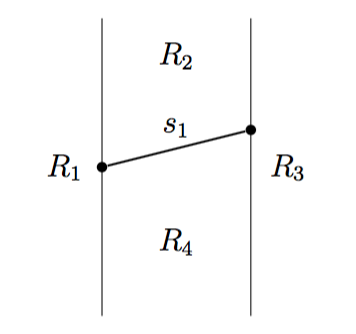
\includegraphics{./immagini/l32-fig2.png}
\caption{Suddivisione di R0}
\end{figure}

Dopodiché viene preso in considerazione il segmento successivo \emph{s2}
e lo utilizziamo per dividere ulteriormente il piano in regioni.

\begin{figure}[htbp]
\centering
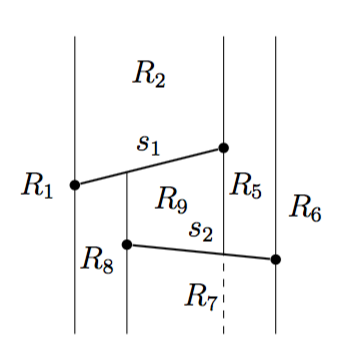
\includegraphics{./immagini/l32-fig3.png}
\caption{Suddivisione con s2, R7 è a cavallo di R3 e R4}
\end{figure}

Da notare che se due parti sono limitate superiormente dallo stesso
segmento, vengono unite in un'unica parte.

Il partizionamento del piano può essere schematizzato in un DAG. Il
grafo ottenuto non è un albero, per il fatto che più parti possono
essere unite in un unica parte.

\begin{figure}[htbp]
\centering
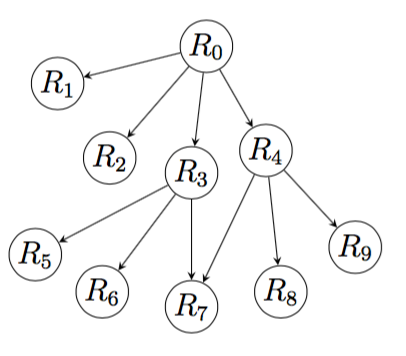
\includegraphics{./immagini/l32-fig4.png}
\caption{DAG rappresentate la suddivisione del piano}
\end{figure}

Una volta suddiviso il piano utilizzando tutti i segmenti si ottiene un
DAG le cui \emph{``foglie''} raprpesentano le regioni del piano e ogni
nodo ha al massimo 4 nodi adiacenti.

Una volta costruito il grafo si parte da \emph{R0} e ci si sposta sulla
regione adiacente al nodo relativo a \emph{R0} e che contiene il punto
\emph{p}.

Per verificare se un punto si trova all'interno di una data regione,
come prima cosa si valuta se la \emph{x} del punto si trova tra
\emph{x1} e \emph{x2}, ovvero le rette verticali che delimitano la
regione. Se il punto si trova tra le due rette, viene verificato con
\texttt{AngleLeft} se si trova sopra il segmento \emph{s1} inferiore
della regione e sotto il segmento \emph{s2} superiore della regione.

Si ha quindi che il test di appertenenza ad una regione può essere fatto
in tempo costante e deve essere ripetuto per ogni regione fino
all'arrivo in una foglia. Nel caso peggiore si ha quindi una complessità
\emph{O(n)}.

\subsubsection{Randomizzazione}\label{randomizzazione}

L'ordine in cui si valutano i segmenti influisce sul partizionamento che
si ottiene, il quale a sua volta influisce sulla lunghezza del cammino
critico del DAG.

\ldots{} Questo cammino prende il nome di \textbf{lunghezza della storia
di \emph{R}}.

Assiumamo quindi che l'ordine di valutazione dei segmenti
\emph{s1,\ldots{}sn} sia casuale e ci chiediamo quale sia la lungehzza
media della storia della regione \emph{R} che cointene il punto
\emph{p}.

\ldots{}
